\chapter{Evaluation}\label{ch:eval}

This chapter evaluates the implementation described in \cref{ch:impl} against the requirements and
threats defined in \cref{ch:threat}. It examines proof size and verification cost, offline catch-up,
scalability, the trade-off between session and continuous modes, comparisons with prior systems, and
the coverage of the security controls.

% ============================================================================
\section{Methodology}\label{sec:eval-method}

The evaluation asks whether detection enlarges an individual proof, how verification changes with
directory size, and whether offline catch-up can use one proof. It also tests whether the defined
attacks are detected and the listed clean workflows complete without warnings. Seventeen metric families connect these
questions to proof size, latency, catch-up, scale, operating modes, and security outcomes.

The Rust harness measures local cryptographic work in process. It excludes HTTP, Electron, database,
and network costs. Manual-harness medians and 95th percentiles use \num{2000} sequential iterations,
while the scale experiment samples \num{1000} lookups per directory size. All DUET timings reported
in this chapter were measured on the Windows x86\_64 host described in \cref{sec:bench-env} (12th Gen
Intel Core i7-12700H, 31.7\,GB RAM). Under the worked parameterization of
\cref{ssec:design-param}, epochs are hourly, so a window of $W=720$ epochs spans 30 days. Proof sizes are exact for the recorded
seeds. Values near timer resolution are treated as coarse observations. Cross-system timing comparisons
are approximate because the published implementations and hardware differ. \Cref{app:benchmarks} defines the metric families
and baseline configurations and provides the complete tables, measurement environment, and
reproduction instructions.

% ============================================================================
\section{Measured Results}\label{sec:eval-micro}

The following subsections present the measured proof sizes and verification costs, offline catch-up
results, and detection-path costs. Each result is stated with the scope of its measurement.


\subsection{Proof Size and Verification (M1--M3, M14)}\label{ssec:eval-sizes}\label{ssec:eval-latency}

A lookup proof carries a prefix copath, a log-inclusion path, and fixed VRF and framing fields. For a
VRF-indexed lookup, its serialized proof body is modelled as:

\begin{equation}\label{eq:eval-proofsize}
  |\pi| \;=\; 32h \;+\; 32h_{\mathrm{log}} \;+\; 177 \ \text{bytes},
  \qquad \mathbb{E}[h]\approx\lceil\lg N\rceil,\quad h_{\mathrm{log}}\le\lceil\lg E\rceil,
\end{equation}

where $h$ is the number of non-empty siblings on the queried label's path and $h_{\mathrm{log}}$ is
the log-inclusion path length. The \num{177}-byte constant comprises the \num{80}-byte ECVRF proof, a
label, a value, a leaf-kind commitment, and a sibling bitmap. Raw-label warning responses omit the VRF
component. The median lookup proof is \num{817} bytes at $N=10^{6}$ and \num{945} bytes at
$N=10^{7}$, and the growth between them is the $\lceil \lg N \rceil$ term, not any change in the
fixed component. The full component breakdown and distribution table are in \cref{sec:bench-sizes}.

Detection does not change this format. A dual-index or CEA check performs another lookup against the
same directory and signed head without enlarging an individual proof.

M14 isolates the history-depth term. Across $E\in\{1,16,256,1024\}$, log inclusion adds
\num{0}, \num{128}, \num{256}, and \num{320} bytes, matching the
$32\lceil\lg E\rceil$ bound. Median full verification remains below
\SI{150}{\micro\second} throughout the grid and reaches at most
\SI{143.2}{\micro\second}. Directory size and history depth therefore contribute independently to
the measured proof size.

Full client verification, which covers the VRF, the log inclusion path, and the signed head, has a
median of \SI{128.7}{\micro\second} at $N=10^{3}$ in the manual harness. Within the scale experiment
(\cref{tab:bench-scale}), the median rises from \SI{133.6}{\micro\second} at $N=10^{6}$ to
\SI{139.2}{\micro\second} at $N=10^{7}$, an increase of \SI{5.6}{\micro\second}, or 4.2 percent, for a
tenfold larger directory. The result supports slow growth relative to directory size. Prefix-only
verification moves from \SI{26.3}{\micro\second} to \SI{26.4}{\micro\second} over the same range,
accounting for little of the full-verification increase. The benchmark does not isolate the remaining
cause.

The 95th-percentile tail for server-side search at $N=10^{7}$ remains unexplained. It is
\SI{4581.9}{\micro\second}, compared with a median of \SI{441.7}{\micro\second}
(\cref{tab:bench-scale}). The harness did not record
operating-system paging activity, so the benchmark cannot determine whether memory pressure caused the
tail. The tail is reported as observed implementation behaviour, without assigning an unmeasured cause.

\subsection{Offline Catch-Up (M4)}\label{ssec:eval-catchup}

A client that has been offline for a window of $W$ epochs must establish that the head it now sees is
consistent with the head it last verified. The windowed construction answers this with one proof
rather than one proof per epoch. At $W = 720$ the windowed proof is \num{320} raw hash bytes against
\num{222528} bytes for the synthetic repeated-proof baseline, a ratio of \num{695.4}.
\Cref{fig:eval-catchup-plot} shows how the two curves separate as the window grows. The baseline is
synthetic and is constructed by repeating the implemented single-epoch proof, so it measures what
this system would cost without windowing, not what any deployed system does cost. Both figures
count raw path hashes and not serialized network traffic. Verifying adjacent epoch transitions would
use smaller individual proofs, so the exact ratio is specific to this baseline even though the
one-proof-versus-$W$-proof comparison remains. Generation timings for the same experiment
are in \cref{sec:bench-sizes}. This addresses the monitoring-bandwidth extension identified by
CONIKS~\cite{melara2015coniks}.

\begin{figure}[ht]
\centering
% fig-eval-catchup-plot.tex — extracted from ch6-evaluation.tex
% Label: \label{fig:eval-catchup-plot}
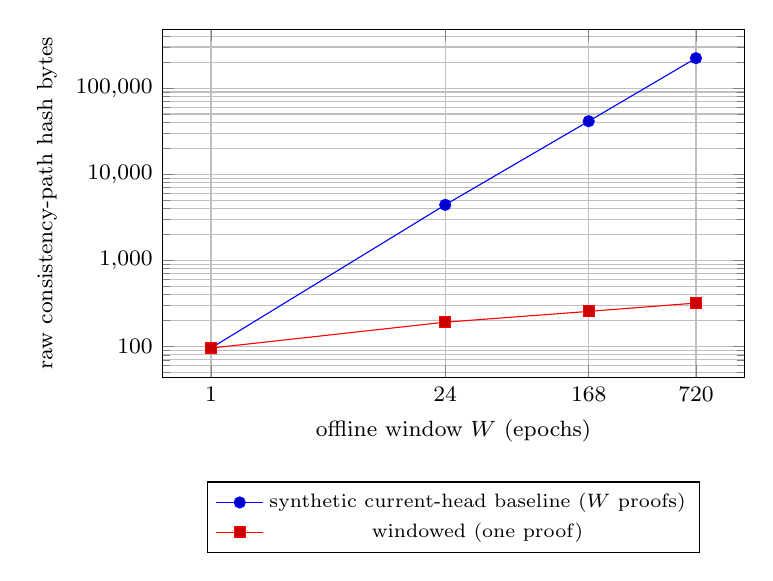
\begin{tikzpicture}
\begin{axis}[width=0.74\textwidth,height=6cm,xmode=log,ymode=log,
  xlabel={offline window $W$ (epochs)}, ylabel={raw consistency-path hash bytes},
  xtick={1,24,168,720}, xticklabels={1,24,168,720}, log ticks with fixed point,
  legend style={at={(0.5,-0.30)},anchor=north,legend columns=1,font=\scriptsize},
  grid=both, font=\footnotesize]
\addplot+[mark=*] coordinates {(1,96)(24,4416)(168,41280)(720,222528)};
\addplot+[mark=square*] coordinates {(1,96)(24,192)(168,256)(720,320)};
\legend{synthetic current-head baseline ($W$ proofs), windowed (one proof)}
\end{axis}
\end{tikzpicture}

\caption[Catch-up bandwidth versus offline window.]{Raw consistency-path hash bytes for offline
catch-up versus window $W$, shown on a logarithmic vertical axis. The synthetic
current-head-anchored baseline grows linearly to \num{222528} bytes at one month. The windowed
proof remains a few hundred bytes and grows logarithmically (\cref{sec:bench-sizes}).}
\label{fig:eval-catchup-plot}
\end{figure}

\subsection{Detection Costs and Clean-Run Results (M16, M17)}\label{ssec:eval-detection}

A verified lookup whose returned owner does not match the expected owner completes in
\SI{27.8}{\micro\second}. The clean two-lookup path fetches and verifies both the self label and the
peer label and completes in \SI{31.1}{\micro\second}. These Rust reconstructions measure local
verified-lookup work in the mismatch and clean paths. They exclude the TypeScript client, transport, polling,
and registration, so they bound the local cryptographic component and do not represent user-visible latency.

All seven specified clean workflows produce their expected clean verdicts (\cref{tab:bench-m17}), and no workflow produces a
warning. The security outcomes are treated in \cref{sec:eval-security}.

% ============================================================================
\section{Scalability, Maintenance, and Authentication Modes}\label{sec:eval-scale}

\subsection{Scale, Maintenance, and Auditing (M7, M9, M12)}\label{ssec:eval-scale}\label{ssec:eval-throughput}\label{ssec:eval-auditor}

Rotation costs between \SI{138.7}{\micro\second} and \SI{140.3}{\micro\second} across the measured
sizes, which is consistent with a fixed-cost VRF dominating the per-label work, not any
dependence on directory size. Epoch commit moves from \SI{451.0}{\micro\second} at $N=10^3$ to
\SI{6.73}{\milli\second} at $N=10^4$. The increase is caused by deep-cloning the current tree into the committed snapshot, not the tree update itself. These two points do not establish an asymptote, but they identify epoch commit as the component
most likely to require engineering attention at deployment scale.

Building the $N=10^{7}$ directory takes about 26 minutes at \SI{21.3}{\giga\byte} resident set on the
evaluation host. The single-process research build holds the whole directory in memory behind one
mutex, making memory use a primary deployment constraint.

M12 measures two local verification operations, not a complete networked audit. The first combines an
STH signature check with consistency-proof generation and verification. Its median is
\SI{28.6}{\micro\second}. This includes proof generation but excludes transport, replay, scheduling,
persistence, and the cross-vantage comparison required by a deployed audit. The second checks for a fork
against one observed head. Its median is \SI{27.1}{\micro\second}, and its 95th percentile is
\SI{33.1}{\micro\second}.

\subsection{Session and Continuous Modes (M13, M15)}\label{ssec:eval-modes}

Session mode and continuous mode show similar isolated label-bound verification cost, at
\SI{27.3}{\micro\second} and \SI{27.7}{\micro\second}. The difference is within run-to-run variation
and no ordering between the two is inferred from it. Verification cost is also stable in the number
of catch-up epochs replayed, varying by at most \SI{0.5}{\micro\second} over
$K \in \{1, 10, 100, 720\}$.

The two modes have similar isolated verification costs, but their write cadences differ. Session mode writes once per
signed-pre-key rotation, while continuous mode writes once per ratchet epoch. At $R = 720$ the
modelled write counts differ by factors between 24 and 720 depending on the modelled number of epochs.
That ratio is a property of the cadence model and the simulated input, and it is not a deployment
bound. The full mode table is in \cref{sec:bench-modes}.

% ============================================================================
\section{Comparison with Prior Systems}\label{sec:eval-compare}

The published systems use different implementations, hardware, and accounting conventions. Each
comparison below therefore states the matched components and arithmetic.
\Cref{tab:eval-compare} summarizes the resulting trade-offs.

\begin{table}[H]
\centering
\caption{DUET compared with prior systems using published figures.}
\label{tab:eval-compare}
\footnotesize
\begin{tabularx}{\textwidth}{@{}>{\raggedright\arraybackslash}p{2.5cm}>{\raggedright\arraybackslash}X>{\raggedright\arraybackslash}X>{\raggedright\arraybackslash}X@{}}
\toprule
Dimension & DUET (measured) & CONIKS~\cite{melara2015coniks} & Signal KT~\cite{signal-kt-server} \\
\midrule
Lookup proof size & 817\,B median at $10^6$ (max 945, prefix and VRF, excluding STH) & 1{,}216\,B at $2^{32}$, 768--832\,B at $10^6$ derived (proof with and without signature) & 8{,}192\,B fixed sibling copath only (256$\times$32, no VRF) \\
Client lookup verification & $\approx$\SI{128}{\micro\second} at $10^3$--$10^4$, \SI{139.2}{\micro\second} at $10^7$ (including VRF and signed-head verification) & \SI{159}{\micro\second} for path verification at $10^7$ and approximately \SI{400}{\micro\second} for signature verification, giving a derived total of about \SI{559}{\micro\second}, excluding VRF & not published \\
Catch-up at $W{=}720$ & 320\,B (1 windowed proof) & $\Theta(W)$, $\sim$530\,kB derived & Monitoring endpoint\newline No published byte figure \\
Key-substitution detection & automatic in-band peer warning (established conversations)\newline global VRF-bound identity check, honest directory (first contact) & manual Safety Number comparison and self-monitoring & optional AKV lookup and self-monitoring\newline no peer warning \\
Authenticated records & Identity-key bindings at global and session-derived slots, and per-epoch ratchet-key fingerprints in continuous mode & Identity-key bindings & Account-identifier, phone-number, and username-hash mappings \\
Query privacy (operator) & No & No & No \\
Resists offline identity recovery (VRF) & Yes (ECVRF, 80\,B) & Yes (discrete-log-based VRF, 96\,B) & Yes (ECVRF) \\
\bottomrule
\end{tabularx}
\end{table}

At $N = 10^{6}$ a CONIKS lookup proof carries a 21-node authentication path, an index or commitment
component, and a signature, which gives $32 \times 21 + 96 + 64 = 832$ bytes, or 768 bytes excluding
the signature~\cite[Section~5.3, Table~1]{melara2015coniks}. DUET's \num{817}-byte median is measured
excluding the signed head, so 768 bytes is the matched quantity, and DUET is within 7 percent of it.
The two systems are therefore in the same size class for an individual lookup, and DUET's detection
capability does not enlarge that individual proof format.

Signal's deployed verifiable key directory verifies a fixed-length prefix copath. Its
\texttt{evaluateProof} routine in \texttt{tree/prefix/verify.go} requires exactly 256 siblings, which
is $256 \times 32 = 8{,}192$ bytes~\cite{signal-kt-server}. Against DUET's \num{817}- and
\num{945}-byte medians the
ratios are 10.0 and 8.7. The difference reflects a trade-off rather than a strict improvement. The fixed-length copath
reveals nothing about how populated the tree is, whereas DUET's bitmap compression exposes
approximately $\lceil \lg N \rceil$ bits of density metadata to whoever holds the proof. DUET
trades that bounded metadata exposure for lower bandwidth. SEEMless reports approximately
8.6\,\si{\kilo\byte} at $N = 10^{7}$ under its own construction~\cite[p.~12]{chase2019seemless}, close
to Signal's fixed \num{8192}-byte copath. The figures are not directly comparable because the
constructions account for different proof components.

For offline catch-up the difference is larger. CONIKS reports an approximately 736-byte per-epoch
proof~\cite[Section~5.3]{melara2015coniks}, so a 720-epoch window costs $720 \times 736 = 529{,}920$
bytes against DUET's \num{320}-byte windowed proof, a ratio of approximately 1{,}656. CONIKS
prescribes a separate proof of the client's binding for every missed epoch. DUET's \num{320}-byte
figure measures the returning client's consistency proof. Peer warnings and transition auditing are
separate mechanisms, and their costs are excluded from this ratio.

For client verification, CONIKS reports a \SI{159}{\micro\second} path verification and an approximately
\SI{400}{\micro\second} signature verification~\cite[Section~5.3]{melara2015coniks}, giving a derived
total of about \SI{559}{\micro\second}. CONIKS publishes no separate VRF timing, so that component is
absent from the total. The matched DUET figure is the \SI{139.2}{\micro\second} full verification at
$N=10^{7}$, aligning the comparison at a large directory size. The proof-size comparison excludes
signed heads and signatures on both sides. The timing comparison includes them on both sides. DUET's
figure includes signed-head verification, and the CONIKS total includes its reported signature
verification.

\begin{quote}\small\noindent\textbf{Comparability note.}
The figures above are drawn from published results measured on different hardware, with different
implementations, and under different workloads. They provide broad context and locate DUET within the
design space. They are not a controlled benchmark, and no claim of superiority
on any dimension other than the stated arithmetic is made.
\end{quote}

% ============================================================================
\section{Security Evaluation}\label{sec:eval-security}

The adversarial suite includes tests for the scenarios defined in \cref{ch:threat}: the honest baseline
A0, key substitution (\hyperref[sc:threat-a1]{A1a and A1b}), warning censorship
(\hyperref[sc:threat-a2]{A2}), network man-in-the-middle (\hyperref[sc:threat-a3]{A3}), split-view
equivocation (\hyperref[sc:threat-a4]{A4}), malicious rotation (\hyperref[sc:threat-a5]{A5}), and the
excluded endpoint-compromise case (\hyperref[sc:threat-x1]{X1}). \Cref{tab:eval-security} summarizes
the attack families, their controls, and the observed outcomes. \Cref{tab:tests-adversarial} records
each scenario individually, and \cref{tab:bench-m17} records the seven clean workflows. Every scenario
produces its expected outcome, and the clean workflows produce their expected clean verdicts with no
warnings.

The test schedule performs one action per epoch, so the table's epoch counts describe the harness
rather than detection latency. The outcomes hold under the assumptions defined in
\cref{sec:threat-assumptions}, in particular an uncompromised endpoint and an auditor with an
independent vantage.

\begin{table}[ht]
\centering
\caption{Evaluated threats, detection controls, evidence, and outcomes.}
\label{tab:eval-security}
\footnotesize
\renewcommand{\arraystretch}{1.3}\setlength{\extrarowheight}{3pt}
\begin{tabularx}{\textwidth}{@{}>{\raggedright\arraybackslash}p{2.0cm}>{\raggedright\arraybackslash}p{3.5cm}X>{\raggedright\arraybackslash}p{3.6cm}@{}}
\toprule
Case & Control and requirement & Evidence & Result \\
\midrule
Key substitution (\hyperref[sc:threat-a1]{A1a and A1b}) & Owner self-check and dual-index warning (G1). & \cref{tab:tests-adversarial}. & Detected. \\
\hyperref[sc:threat-a3]{A3} network MitM postcondition & Global VRF-bound identity check, honest directory (G1). & \cref{tab:tests-adversarial}. & Detected at the next lookup. \\
\hyperref[sc:threat-a5]{A5} malicious rotation & Identity re-fetch and predecessor cross-signature (G1). & \cref{tab:tests-adversarial}. & Detected. \\
\hyperref[sc:threat-a2]{A2} warning censorship & Pre-commit key mismatch with proof-verified warning absence, and post-commit removal caught as an invalid transition (extension of G1). & \cref{tab:tests-adversarial}. & Detected. \\
\hyperref[sc:threat-a4]{A4} split-view equivocation & Cross-vantage auditor (G4). & Equivocation test and the M12 signed-head fork comparison. & Detected at the next comparison. \\
\midrule
Offline identity recovery from published labels (G3) & ECVRF-derived labels resist offline recovery of identities by traversing public labels (G3). & VRF assumption. RFC~9381 vectors check implementation conformance (\cref{tab:tests-rust-prim}). & Resisted offline under the VRF assumption. The public query endpoint still permits online membership tests. \\
\hyperref[sc:threat-x1]{X1} key extraction & No directory control. & Endpoint compromise lies outside key transparency. & Out of scope. \\
\bottomrule
\end{tabularx}
\end{table}

The supporting analysis maps the scenarios to STRIDE~\cite{stride} in
\cref{sec:sec-stride}, MITRE ATT\&CK~\cite{mitre-attack} in \cref{sec:sec-mitre},
and the attack routes in \cref{sec:sec-routes}, while \cref{ssec:eval-timeline}
gives the detection sequence.

\subsection{Residual Risks and Security Position}\label{ssec:eval-posture}

A rejecting verdict shows that an integrity or consistency check failed without identifying its cause
or attributing it to the directory operator. An unavailable directory server raises an amber notice,
while a verified mismatch or the fail-closed operational timeout raises a red
warning. Endpoint compromise defeats every mechanism evaluated here because the verifier and the keys
it trusts live on the endpoint.

% ============================================================================
\section{Implications for Deployment}\label{sec:eval-deploy}

The measured client costs support the feasibility of client-side verification at the tested scale:
median full verification stays below \SI{150}{\micro\second} through $10^7$ labels, the proof body
stays below one kilobyte, and detection reuses this format through additional label-bound lookups
without enlarging an individual proof.

Offline catch-up uses one proof for the missed window. At $W=720$, its \num{320} raw hash bytes
compare with \num{222528} bytes across \num{720} proofs for the synthetic repeated-proof baseline.
Both figures exclude serialization overhead. The baseline models this implementation without
windowing, not a deployed system.

M16 measures the Rust lookup work for the mismatch path and the clean two-lookup path. These
component timings exclude network transfer and end-to-end background-monitor latency. The directory server measurements expose two
further constraints. Epoch commit deep-clones the current tree into the committed snapshot, and the
in-memory tree becomes large at $10^{7}$ entries. Persistent structural sharing, storage, concurrency
testing, and networked measurements remain necessary.

Session and continuous modes have similar isolated verification costs but different write frequencies.
Their measured ratio reflects the cadence model, not a fixed deployment value.
